\section*{הקדמה}
\begin{displayquote}
אלגוריתם הוא דרך שיטתית (כלומר כזו שצעדיה מוגדרים היטב) לביצוע של משימה מסוימת, 
במספר סופי של צעדים.
\end{displayquote}
\leftline{\textenglish{---} \textit{ויקיפדיה}}
המושג אלגוריתם אינו חדש עבורנו, ראינו ומימשנו כבר אלגוריתמים בקורס מבוא למדעי המחשב, 
מבוא לתכנות מערכות ומבני נתונים.
\subsection*{חשיבות הקורס}
בתעשייה - בעיות שמצריכות פתרון אלגוריתמי צצות במגוון תחומים. על פי
\textenglish{glassdoor}, 
מפתח אלגוריתמים מרוויח 20 אחוז יותר מאשר מהנדס תוכנה.
\\
במחקר האקדמי - חלק עיקרי של המחקר האקדמי הוא בפיתוח וניתוח אלגוריתמים.
\subsection*{חומר הקורס}
בקורס נלמד מגוון אלגוריתמים שעל פי רוב נחשבים לבסיס בתחום האלגוריתמים.
הרוב המוחלט של האלגוריתמים שנלמד בקורס הם אלגוריתמים על גרפים 
וזאת מכיוון שגרפים הוכיחו את עצמם ככלי מאוד חזק בייצוג מגוון רחב של בעיות.
לחלק מהאלגוריתמים שימושים ברורים (מסלול קצר ביותר, עצי הופמן), 
חלק מהאלגוריתמים מהווים פתרון למגוון גדול של בעיות שניתנות לייצוג בצורה מסוימת (זרימה), 
וחלק מהאלגוריתמים מהווים בסיס לפיתוח אלגוריתמים מורכבים יותר (%
\textenglish{BFS},
\textenglish{DFS}, 
עץ פורש).
מעבר לזה נלמד טכניקות (פשוטות יחסית) כלליות לפיתוח אלגוריתמים.
\section*{סריקת גרפים}
\begin{example}
רוצים למצוא (ולהדפיס) את כל קבצי התמונות ששמורות על הכונן הקשיח.
\end{example}
למשל עבור:
\begin{center}
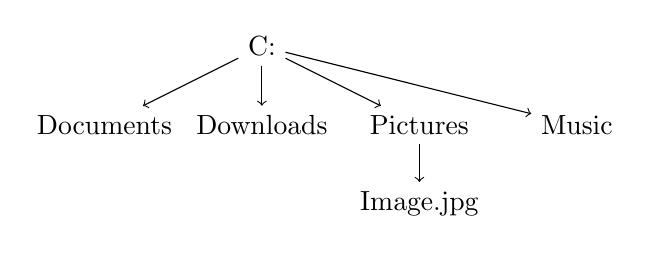
\begin{tikzpicture}[every node/.style={rectangle}, ->]
\node(00) at(0,0) {\text{C:}};

\node(10) at(-2, -1){\text{Documents}};
\node(12) at(0, -1){\text{Downloads}};
\node(13) at(2, -1){\text{Pictures}};
\node(14) at(4, -1){\text{Music}};

\node(21) at(2, -2){\text{Image.jpg}};

\foreach \v in {10,12,13,14}{
	\draw (00) -- (\v);
}
\draw (13) -- (21);

\end{tikzpicture}
\end{center}

כיצד עלינו לסרוק את מערכת הקבצים ? 
\begin{enumerate}
\item
במידה ורוצים להדפיס את (הנתיב המלא של) הקבצים בסדר לקסיקוגרפי ?
\item
במידה ורוצים להדפיס קבצים לפי העומק שלהם (מספר תיקיות) ?
\end{enumerate}
נשים לב שאפשר לייצג את מערכת הקבצים באמצעות גרף מכוון (ברוב מערכות הקבצים עץ אינו ייצוג מספק)
ולכן נעביר את הדיון שלנו לסריקת גרפים.

\subsection*{ייצוג גרפים}
קיימים שני ייצוגים סטנדרטים של גרפים (מכוונים או לא):
\begin{enumerate}
\item
על ידי מטריצת שכנויות
\item
על ידי רשימת שכנויות
\end{enumerate}

אם לא מצוין אחרת, נניח שהגרף מיוצג על ידי רשימת שכנויות.
\subsection*{אלגוריתם כללי}

